
% 原文 p.329
\hypertarget{srcpage:329}{}\label{srcpage:329}
\sectionlink{量子力学の解釈におけるデコヒーレンスの役割}
\setcounter{footnote}{0}

物理学者の精鋭たちが量子力学の解釈について激しい議論を交わした、1927年の有名なSolvay会議\cite{ref385}から、すでに何十年もの歳月が過ぎた。それでも、量子論の意味をめぐる議論には衰える兆しがない。量子力学に対する純粋に実用主義的な「黙って計算せよ」という姿勢\footnote{この呼称はしばしばFeynmanに帰されるが、「黙って計算せよ解釈」というあだ名を実際に作ったのはMermin\cite{ref386}らしい。このような解釈上の立場の例として\cite{ref044}を参照されたい。}を超え、量子形式と、私たちの「外部」にあると想定される物理的実在とを結びつけようとすれば、解釈の問題に巻き込まれることはほとんど避けられない。したがって、多様な量子力学の解釈の存在は、量子論そのものと同じくらい古い。

本章では、次の重要な問いを論じる。デコヒーレンス自体が量子力学の解釈上の問題と関係していることを踏まえると、デコヒーレンスはこれらの異なる解釈にどのような含意を持つのだろうか。この問いは、とりわけ興味深い。というのも、相対状態解釈、様相解釈、de BroglieとBohmのパイロット波理論など、主要な解釈の多くがすでに定式化されてから、かなり後になってデコヒーレンスが「発見」されたからである。（第1章の末尾で述べたように、デコヒーレンスが科学者の共同体から広く注目され始めたのは、1990年代の初めになってからにすぎない。）量子測定のような解釈に関係する主題を現実的に記述するうえで、デコヒーレンスが重要であるとようやく認識されると、既存の、また将来の量子力学の解釈に対するその含意を問うことが、切実な意味を持つようになった。解釈の主要な目的の一つは量子測定の不可解な側面を理解することであり、デコヒーレンスは、とりわけそのような測定の現実的な記述を扱っていた。したがって、デコヒーレンスから得られた新しい知見を踏まえて、これらの解釈を再検討することは避けられなかった。

量子力学の解釈に対するデコヒーレンスの含意を調べる際に出会う、いくつかの重要な問いを挙げよう。

% 原文 p.330
\hypertarget{srcpage:330}{}\label{srcpage:330}
\begin{itemize}
\item デコヒーレンスだけで量子力学の基礎に関する特定の問題を解決し、個々の解釈が量子力学に導入した解釈上ないし形式上の付加物の一部を不要にできるだろうか。もしできるなら、どのような核心的な基礎問題が残り、それらはどのような形を取るのだろうか。
\item デコヒーレンスは解釈の経験的適合性を保証できるだろうか。すなわち、ある解釈が実験によって反証されるのを防ぐことができるだろうか。
\item 逆に、デコヒーレンスは、ある解釈が標準量子力学や観測と衝突することを示すことによって、その解釈を排除できるだろうか。
\item デコヒーレンスは、個々の解釈が導入する仮定の一部に物理的な動機を与え、それによって、それらの仮定にいっそう明確な物理的意味を与えることができるだろうか。
\item デコヒーレンスは、さまざまな解釈を統合し簡素化する「融合剤」として、どの程度まで働くことができるだろうか。そうすることで、一見異なる解釈を共通の核心へ還元できることを示せるだろうか。
\end{itemize}
本章では、これらの問いやほかの問いを、量子力学の主要な解釈の流れごとに取り上げ、分析する。本章の一部は、著者の総説\cite{ref001}\footnote{本章の一部は、許可を得て\cite{ref001}を改作したものである。Copyright 2004 by the American Physical Society.}に基づいている。標準解釈とCopenhagen解釈（8.1節）、相対状態解釈（8.2節）、様相解釈（8.3節）、物理的収縮理論（8.4節）、Bohm力学（8.5節）を考察する。これによって、デコヒーレンスに照らして異なる解釈の現状を評価できるだけでなく、デコヒーレンス自体の意味と適用範囲についても、新しい知見が得られるだろう。

\subsectionlink{標準解釈とCopenhagen解釈}
本節では、量子力学の教科書の大部分で、明示的または暗黙的に示されている標準解釈を論じる。この解釈は、量子力学の「正統的」解釈とも呼ばれることが多い。ここでは、標準解釈とCopenhagen解釈\footnote{実際には、単一で首尾一貫した「Copenhagen解釈」は存在せず、Bohr、Heisenbergおよび同時代の人々による、時には食い違う見解の寄せ集めであることが指摘されており\cite{ref387}、現在では広く認識されている。ここでの議論は、BohrとHeisenbergが提起した解釈上の考え方を指すものとする。ただし、両者の考え方を区別する必要がある場合も多い。}を意識的に区別する。後者は、測定を含む量子現象を記述するために、基本的で還元不可能な古典的概念が必要であるという追加の仮定を導入するからである。
% 原文 p.331
\hypertarget{srcpage:331}{}\label{srcpage:331}
Copenhagen解釈のこの特徴には、後の8.1.3節で立ち戻る。Copenhagen解釈とデコヒーレンスの関係に関する詳しい議論は\cite{ref388}にある。\cite{ref389,ref390}も参照されたい。

標準解釈を特徴づけるのは、本書のさまざまな箇所ですでに触れた収縮公準である。この公準はいくつかの部分に分けられる。第一に、量子系に対して行われるすべての測定は、ユニタリーな時間発展に不連続な中断を生じさせる。第二に、この中断によって、測定される観測量の固有状態で展開された波動関数が、それらの項の一つへ「収縮」する。こうして、重ね合わせの一成分が測定結果として選ばれる。第三に、ある特定の結果の確率は、初期波動関数と、その結果に対応する量子状態との重なりの振幅の絶対値の二乗で与えられる（Born則。原著35頁の脚注9も参照）。

標準解釈は、収縮の本性について何の説明も与えない\footnote{他方、Copenhagen解釈は、収縮の認識論的性格を強調しているように見える。この解釈では波動関数を確率振幅だけを表すものとみなすため、収縮は実際の物理過程というよりも、単なる「情報の増加」という性格を持つ。2.1節の議論も参照されたい。}。この解釈における測定と収縮公準の際立った役割にもかかわらず、「測定」の具体的な定義はかなり不明確なままである。原理的には、標準解釈は「古典的」状態の巨視的重ね合わせの可能性を、あらかじめ排除しない。同時に、そのような重ね合わせを観測する行為は、収縮を引き起こす測定相互作用にほかならないから、決して観測できないともいう。しかし、厳密に何が測定に当たるのかという問いには、答えが与えられない。収縮を引き起こすには人間の観測者が必要なのだろうか。ある相互作用はいつ収縮を引き起こし、いつ系がユニタリーに発展し続けることを許すのだろうか。

\subsubsectionlink{結果の問題}
結果の問題は、von Neumannの測定図式との関連ですでに論じた（2.5.4節参照）。そこで述べたように、標準解釈では、結果、すなわち確定した「値」の存在に関する解釈規則は、固有値・固有状態リンクによって与えられる。この規則は、系がある物理量について確定した値を持つのは、その物理量に対応する観測量の固有状態にある場合、かつその場合に限ると定める。これは「客観的な」基準である。なぜなら、ある物理量の値を帰属させられる、系の確定した量子状態の存在を推論できるからである。

この解釈の枠組みの中では、収縮公準を前提としない限り、デコヒーレンスは2.5.4節で述べた結果の問題を解決できない。
% 原文 p.332
\hypertarget{srcpage:332}{}\label{srcpage:332}
巨視的に異なる指針状態間の位相コヒーレンスは、環境を含む状態では保存されており、系を拡大して環境の少なくとも一部を含めることが、いつでもできるからである。言い換えれば、コヒーレンスが環境へ非局在化することによって、重ね合わせが拡大されるだけであり（「干渉項は依然として存在するが、そこにはない」\cite[224頁]{ref007}）、デコヒーレンス過程は原理的には常に逆転できる。したがって、物理量の確定した値の存在を正統的な固有値・固有状態リンクで確立すると仮定するなら、デコヒーレンスは、系が実際にいつか一つの確定した指針状態にあることも、そもそも測定に結果があることも保証できない。もちろん、系が初めから指針観測量の固有状態にある場合は別である。

この重要な点を、もう少し詳しく論じよう。まず、全体の系・環境量子状態ベクトルについていえば、環境との相互作用はもつれを追加しただけであることに注意しよう。
\begin{equation}
|\Psi(t=0)\rangle=\Bigl(\sum_n c_n|s_n\rangle\Bigr)|E_0\rangle
\longrightarrow |\Psi(t)\rangle=\sum_n c_n|s_n\rangle|E_n(t)\rangle .\tag{8.1}
\end{equation}
ある意味では、環境との相互作用が生み出すもつれは、von Neumann図式で考えられる測定問題（2.5節参照）を、最初はかえって悪化させるとさえ考えられる。Bacciagaluppi\cite[3.2節]{ref391}は、この点を次のように述べている。
\begin{quote}
直観的には、環境が私たちの介入なしに多数の近似的な位置測定を行っているなら、測定問題は、そのように自発的に起こる測定にも、より広く当てはまるはずである。（中略）物体と環境の状態は、非常によく局在した無数の項の重ね合わせとなり得る。それぞれの項はわずかに異なる位置にあり、それら全体は、日常的な物体の場合でさえ、巨視的な距離にわたって広がっている。（中略）あらゆるものがほかのあらゆるものと相互作用しているなら、あらゆるものがほかのあらゆるものともつれていることになり、それは測定装置と測定対象のもつれよりも悪い問題である。
\end{quote}
環境の相対状態の重なり$\langle E_n(t)|E_{m\ne n}(t)\rangle$が急速に減少すること、すなわちそれらの状態の識別可能性が増すことが意味を持つのは、量子力学の通常の測定公理に基づいて局所測定を考えるようになってからである。たとえば、状態(8.1)に対応する系の縮約密度行列を作ると、
\begin{equation}
\hat\rho_{\mathrm S}(t)=\sum_{mn}c_m c_n^*|s_m\rangle\langle s_n|\langle E_n(t)|E_m(t)\rangle .\tag{8.2}
\end{equation}
2.7節で論じたように、重なり$\langle E_n(t)|E_{m\ne n}(t)\rangle$の急速な減衰は、干渉項$|s_m\rangle\langle s_{n\ne m}|$が抑制されることを意味する。
% 原文 p.333
\hypertarget{srcpage:333}{}\label{srcpage:333}
縮約密度行列は、成分状態$|s_n\rangle$の、近似的ではあるが非真正の集団へ変わる。
\begin{equation}
\hat\rho_{\mathrm S}(t)\approx\sum_n|c_n|^2|s_n\rangle\langle s_n| .\tag{8.3}
\end{equation}
縮約密度行列を導入した動機は、この数学的対象が局所系のすべての測定統計を完全に含んでいるという事実であったことを思い出そう。これらの統計は、可能なすべての局所観測量$\hat O_{\mathrm S}$の期待値によって与えられ、トレース規則$\langle\hat O_{\mathrm S}\rangle=\operatorname{Tr}(\hat\rho_{\mathrm S}\hat O_{\mathrm S})$から計算される。実用上あらゆる目的について、また系だけに対するいかなる局所測定についても、系の縮約密度行列(8.3)が生成する統計は、それに対応する純粋状態の真正混合、すなわち集団が生成する統計と、近似的に同じになる。この純粋に操作的な意味で、デコヒーレンスは、特に巨視的領域において、ある種の干渉効果がなぜこれほど観測しにくいのかを説明する（2.7節と2.5.3節も参照）。

しかし、トレース操作は非ユニタリーであり、一般には測定の異なる結果についての平均という動機と解釈を与えられていることに注意しよう。2.4.1節で示したように、形式的な式$\operatorname{Tr}(\hat\rho\hat O)$を、演算子$\hat O$が表す量の期待値と同定する根拠は、次の数学的事実にある。このトレースを書き下すと、$\hat O$が表す測定の可能な結果について、それぞれの結果に対応する特定の状態へ測定中に系が「投げ込まれる」Born確率で重みをつけた和と等しくなるのである。しかしこの解釈は、測定に結果があり、Born則が成り立つことを、すでに前提としている。したがって、トレース操作、そして縮約密度行列の概念とその解釈は、統計的解釈と、量子力学の通常の測定公理に基づいている。Pessoa Jr.\cite[432頁]{ref064}の言葉では、「部分トレースを取ることは、射影公準の統計的な形に相当する」。

量子力学の標準解釈において、結果の存在を保証し、それゆえ系へ物理量の確定した値をいつ割り当てられるかを定めるのは、まさにこの射影公準、すなわち収縮公準である。したがって、縮約密度行列のように、トレース規則によって得られる形式的構造から、その結果の存在を導くことはできない。測定公理、したがってトレース規則を取り去ると、残るのは全体の系と環境がもつれた状態(8.1)である。標準解釈によれば、この状態からは系の物理状態について何もいえず、特定の結果、すなわち物理量の確定した値を、系へ割り当てることもできない。


% 原文 p.334
\hypertarget{srcpage:334}{}\label{srcpage:334}
\subsubsectionlink{観測量、測定、環境誘起超選択}
標準解釈とCopenhagen解釈では、物理的性質の割り当ては、ある物理量の測定を表す観測量によって定められ、その観測量が優先基底を定義する。しかし、任意のHermite演算子が観測量の役割を果たせるから、どのような状態も、無限個の異なる性質を潜在的に持っている。それらの性質の帰属は通常、相互排他的である。ただし、対応する観測量が可換な場合は別であり、その場合は共通の固有基底があるため、優先基底の一意性が保たれる。それでは、測定される観測量を何が決めるのだろうか。標準解釈とCopenhagen解釈では、本質的には「利用者」が、測定する特定の観測量を単に「選び」、それによって系がどの性質を持つかを決めるのである。

この実証主義的な見方は、多くの論争を生んできた。それは、自然科学が始まって以来その核心をなしてきた、観測者に依存しない実在という考えに反する。さらに、実際には、任意の観測量を自由に選んで測定できるわけではない。私たちが持つのは、特定の観測量を測定するように作られた、感覚器官をも含む「装置」である。ほとんどの、そしておそらくすべての実用的目的について、これは最終的には一つの関係する観測量、すなわち位置に帰着するだろう。しかし、装置を特定の観測量に適したものにしているのは何だろうか。

この決定的な問いに答えるには、実際の物理的測定の仕組みと、仮にあってもわずかな関係しか持たない「ブラックボックス」過程として測定を扱う、正統的な見方を本質的に捨てなければならない。測定を、系と装置の間に量子相関が形成されることとして形式化する考えは、量子力学の初期にさかのぼり、von Neumannの測定図式にも表れている（2.5.1節参照）。しかし、2.5.2節で論じたように、それだけでは、観測量がどのように選ばれるかという問題は解決しない。第二の要素、すなわち測定過程の記述に環境を明示的に含めることは、デコヒーレンスの研究によって量子論へ持ち込まれた。Zurek\cite{ref008}が導入した指針状態の安定性基準は、測定が頑健な記録を確立するような性質を持たなければならないことを意味する。すなわち、周囲の環境との避けられない相互作用にもかかわらず、系と装置の相関が保存されなければならないのである（2.8節の議論参照）。「利用者」は観測量を任意に選ぶことはできず、環境との相互作用が安定した記録を保証するような測定装置を設計しなければならない。それによって、その観測量に対する測定装置が定義される。正統的量子力学の読み方では、これは環境が系の性質を決定していると解釈できる。

この意味で、デコヒーレンスの研究計画は、標準解釈とCopenhagen解釈が提起する、観測者が自由に選ぶように見える観測量という曖昧な概念を伴った、かなり形式的な測定概念を、より現実的で物理的な動機を持つ枠組みへ組み込んだ\cite{ref388}。
% 原文 p.335
\hypertarget{srcpage:335}{}\label{srcpage:335}
これは、測定装置の物理的構造と環境との相互作用を考慮し、測定される観測量を選ぶための、観測者を必要としない基準を指定することによって実現される。ほとんどの場合、測定記録を増幅し\cite{ref076}、それによって外部観測者が利用できるようにするためにも、環境が必要である（2.9節も参照）。

\subsubsectionlink{Copenhagen解釈における古典性の概念}
Copenhagen解釈は、さらに、古典性は量子力学から導かれるべきものではないとする。たとえば、基礎にある量子構造の巨視的極限として導くべきものではない。標準解釈では、ある意味でそう仮定しているが、明示的には導いていない。代わりにCopenhagen解釈は、古典性を完全な量子論の不可欠で還元不可能な要素、さらには量子論に先立つ概念とみなすべきだと定める。特に、古典物理学に従い、量子力学的には記述すべきでない巨視的測定装置の存在を仮定する。この点はvon Neumannの測定図式と著しく対照的である。そのような古典的装置は、私たちの経験する「古典的」世界の言葉で量子力学的現象に接近するために必要だと考えられる（たとえば\cite[209頁]{ref072}参照）。量子力学で記述すべき系と、古典物理学に従う装置とのこの二元論は、系と装置の間に、原理的には移動可能であるとはいえ、基本的な境界が存在することも意味する。その境界は微視的世界を巨視的世界から分ける（「Heisenberg切断」\cite[15頁]{ref392}）\footnote{\cite{ref388}で詳しく論じられているように、BohrとHeisenbergは、切断についてかなり異なる考えを持っていたようである。特にHeisenbergは、切断の位置は「物理的に確定することができない」、それは物理的不連続を表すものではない\cite[49頁]{ref393}とし、「しかも、切断の位置を選ぶ際の恣意性こそが、量子力学の適用にとって決定的なのである」\cite[416頁]{ref394}と述べた。これに対し、Heisenberg\cite[24頁]{ref395}が回想するところでは、「Bohrは、対象と残りの世界との分割は任意ではないと述べる方が、より現実的であることを強調していた」のであり、対象は実験自体の本性によって定まる。Howard\cite{ref396}も、Bohrにとって量子・古典の区別は、対象・装置の区別と厳密に一致してはいなかったのに対し、Heisenbergにとっては、まさに一致していたように見えると論じている。}。

Bohr、Heisenbergたちが「還元不可能な古典的概念」の必要性を主張したとき、厳密に何を意味したのかを理解することは、難しいことで知られる。詳しい議論については、たとえば\cite{ref388,ref396}を参照されたい。デコヒーレンスによる古典性の創発という研究計画に照らして、そのような古典的概念の基本的な考え方が不要になるのか、あるいは維持不能にさえなるのかは、それらの概念に認識論的、物理的といったどのような地位を与えるかに、大きく依存する\cite{ref388}。
% 原文 p.336
\hypertarget{srcpage:336}{}\label{srcpage:336}
明らかなのは、環境誘起超選択と干渉の抑制が、量子形式だけを用い、微視的尺度から巨視的尺度までの広い範囲にわたり、準古典的で頑健な状態がどのように出現し、あるいは出現しないままでいるかを示してきたことである。これは、系と装置との境界を、かなりの程度まで装置の側へ動かせることを示す近年の実験（第6章参照）と、非常によく一致している。同様の結果は、環境による系の監視を含む、量子非破壊測定の一般的研究からも得られている（たとえば\cite{ref138}の第19章参照）。このように、デコヒーレンスはHeisenberg切断の位置を一義的に指定し、量子・古典の区分と、その境界における動力学に、物理的で定量的な基盤を与える。

Copenhagenの見方では、装置は古典的に記述されるので、定義上巨視的だということに注意しよう。しかし、実際の「計器」は、微視的であってもよい。巨視的でなければならないのは、測定記録の実効的な不可逆性と冗長性を保証する「増幅器」だけである。この点を最初に強調したのはZurek\cite{ref076}である。\cite{ref016,ref323,ref389}における彼の議論も参照されたい。例として、2.10節で述べたデコヒーレンス模型を考えよう。ここでは、系は二安定原子で表された「計器」に対応し、環境が増幅器の役割を果たす（「ビットをバイトで測定する」）。同様に、ある種の巨視的測定装置も、「微視的な」量子力学的言葉で記述できる。例として、重力波の巨視的検出器\cite{ref069}や、量子限界における位置測定\cite{ref310}を実現するための、量子電気機械系\cite{ref307}における巨視的共振器がある（6.4.2節参照）。どちらの装置も、量子力学的調和振動子として扱うことができる。

デコヒーレンスの研究計画がすでに達成した進歩に基づけば、何らかの追加的な解釈構造に組み込まれたデコヒーレンスによって、量子力学的原理から古典世界の現れを、完全かつ整合的に導けるようになると予想するのは合理的である。物理的な観点からは、量子力学の領域外で扱わなければならない、本質的に古典的な装置を仮定することは、必要でも実行可能でもないように見えるだろう。このようにして、古典世界の必要性というBohrの認識論的考えの正しさを認めると同時に、古典世界を、純粋に量子力学的な基盤の一部であり、そこから出現するものとみなすことができる\cite{ref067,ref104,ref388,ref391}。

\subsectionlink{相対状態解釈}
正統的量子力学の系・観測者二元論は、量子系の決定論的法則で記述されず、代わりに確率的な非決定性に従う、外部の「観測者」を理論へ導入する。この方法は、宇宙全体を考えると、明らかに問題に突き当たる。定義上、外部の観測者は存在できないからである。


% 原文 p.337
\hypertarget{srcpage:337}{}\label{srcpage:337}
相対状態解釈の中心的考えは、この系・観測者二元論を捨てることである。この考えは1950年代末にHugh Everett\cite{ref140}が初めて述べ、ただし詳細には展開せず、その後多くの著者が発展させた。代わりに、(i)宇宙全体の物理状態を表す全量子状態$|\Psi\rangle$の存在を仮定し、(ii)Schrödinger発展の普遍的妥当性を維持する。さらに、(iii)測定終了時に、全状態を測定観測量の固有基底で展開したすべての項が、ある意味で物理状態に対応すると仮定する。すなわち、形式上も物理上も、特定の「結果」は選ばれない。これらの各物理状態は、(a)複合系の他方の部分の状態に対して相対的なもの（Everettの原案。\cite{ref141,ref143}も参照）、(b)絶えず「分裂」する宇宙のある「分枝」に対して相対的なもの（DeWitt\cite{ref397}とDeutsch\cite{ref398}が広めた多世界解釈）、あるいは(c)意識的観測者の心の集合における、特定の「心」に対して相対的なもの（多心解釈。たとえば\cite{ref399}参照）と理解できる。

相対状態解釈は、二つの大きな困難に直面する。第一は優先基底問題である。状態が相対的なものにすぎないなら、何に対して相対的なのかという問いが生じる。分枝を定義するために使われ、次の瞬間に相対的な性質、世界、心を指定する、特定の基底項を何が決めるのだろうか。「分裂」は厳密にいつ起きるのか。それぞれの分枝でどの性質が確定し、それらは私たちが経験する確定した性質とどのようにつながるのか。第二に、可能なすべての結果がある意味で「起こる」なら、確率は何を意味し、そのような解釈の枠組みでBorn則をどのように動機づけられるのか。以下で述べるように、相対状態解釈の支持者は、これらの困難を解決するため、しばしばデコヒーレンスに訴えてきた（たとえば\cite{ref398,ref400,ref401,ref402,ref403,ref404,ref405,ref406,ref407}参照）。

他方、ZehやZurekのようなデコヒーレンス研究の先駆者も、Everettの相対状態の枠組みの考え方を、しばしば利用してきた（たとえば\cite{ref004,ref005,ref104,ref408}参照）。これはおそらく、Everettの方法が、解釈上の追加要素を最小限にして、ユニタリー量子力学を本質的に「そのまま」受け入れるためだろう。この姿勢は、基本的な量子力学の形式だけから古典性の出現を説明しようとする、デコヒーレンス研究の精神によく合う。Zehは、異なる観測者が付随するEverett型の分枝を支持している\cite{ref408}（9.4節も参照）。Zurekは、優先基底問題を明確に示し\cite{ref008}、安定な測定記録の重要性と役割を強調する\cite{ref084,ref104}ために、相対状態を有用な概念として用いた（後の8.2.3節で述べるZurekの「実存的解釈」参照）。

\subsubsectionlink{Everett分枝と優先基底問題}
Stapp\cite[1043頁]{ref409}は、「量子論の多世界解釈が存在するのは、付随する基底問題が解決される限りにおいてのみである」という要件を述べた。
% 原文 p.338
\hypertarget{srcpage:338}{}\label{srcpage:338}
相対状態解釈では、優先基底問題は正統的解釈におけるよりもはるかに深刻であるだけでなく、少なくとも次の二つの理由によって、より根本的でもある。
\begin{enumerate}
\item 分枝は連続的に、しかも本質的にあらゆる場所で起こる。測定を量子相関の形成という一般的な意味で理解するなら、新たに形成される相関は、微視的な系に関するものであれ巨視的な系に関するものであれ、すべて分枝に対応する。
\item 少なくとも世界や心の実際の「分裂」を仮定する相対状態解釈では、存在論的含意ははるかに劇的である。基底の選び方が、結果として生じる「世界」や「心」全体を決めるからである。
\end{enumerate}
デコヒーレンス研究における環境誘起超選択の基準は、相対状態解釈の優先基底問題を解くために、しばしば利用されてきた（たとえば\cite{ref104,ref406,ref407,ref410}参照）。デコヒーレンスに基づいて優先的なEverett基底を選ぶ方法には、いくつかの利点がある。第一に、優先基底の存在をあらかじめ仮定する必要がなく、頑健性という物理的基準から、優先基底が動力学的に生じる。第二に、デコヒーレンスの研究計画は、よく検証されたSchrödinger動力学だけから導かれるため、この選択は経験的に適切である。ただし、頑健性が普遍的に妥当な選択基準ではない可能性は別に考慮する必要がある。最後に、発展する波動関数のデコヒーレンスした成分を、時間を通じて再同定できる。それらは優先状態空間の「軌道」を形成し、安定で時間的に持続するEverett分枝を定義するために使える。同様に、そのような軌道を観測者の頑健な記録状態や、系の状態についての情報を多くの観測者が利用できるようにする環境状態へ対応させることもできる（2.9節、および後の8.2.3節参照）。

環境誘起超選択とデコヒーレンスによってEverett分枝を定義する方法は、「概念的に近似的」であるとして批判されてきた。環境誘起超選択は、一般に優先基底を近似的にしか指定しないので（2.8.3節参照）、Everett分枝の「厳密な」定義を与えられないからである（たとえばKentのコメント\cite{ref411}、およびBellの論考\cite{ref412}参照）。Wallace\cite[90--91頁]{ref407}は、このような反論は、
\begin{quote}
（前略）Everett型解釈についての多くの議論に暗黙に含まれる、ある見方から生じている。すなわち、量子力学におけるある種の概念や対象は、理論の公理的構造へ形式的に組み込まれるか、さもなければ幻想とみなされるしかない、という見方である。（中略）［これに対して］量子力学からの古典世界の出現は、ある種の構造とパターンが理論から出現することとして理解すべきである。そして……これは、Kent\cite{ref411}たちが要求するような精密さが、必要でもなければ、望みようもないことを意味する。
\end{quote}
と論じた。


% 原文 p.339
\hypertarget{srcpage:339}{}\label{srcpage:339}
実際、優先基底の選択における「近似的な」基準が、経験的に適切で、私たちの経験を説明するEverett分枝の有意味な定義を与えられることを、あらかじめ疑う理由はないとするのは合理的である。環境によって超選択された基底は、物理的に非常にもっともな頑健性の基準と、純粋に量子力学的なデコヒーレンスの効果から現れる。公理的に導入した「厳密な」規則が、同じように物理的な動機を持ち、経験的適合性を保証できる仕方で、優先基底を選べるとは、むしろ想像しにくい。

環境によって超選択された指針状態でEverett分枝を記述するほかに、複合状態の各瞬間のSchmidt分解、あるいはそれと等価な、縮約密度行列の直交固有状態の集合を、優先基底の定義に直接用いる著者もいる（Schmidt分解は2.15.1節で論じた）。この方法では各瞬間の単純な数学的対角化から優先基底が直接得られるので、動力学的に安定な指針状態を明示的に探索するよりも実行しやすい。また、相対状態解釈における基底選択の「厳密な」規則も与える。Schmidt分解が量子論に由来し、量子力学の形式がそれ自体の解釈を与えるというEverettの提案の「純粋な量子力学」の精神によく合うことも、利点に数えられてきた\cite{ref147}。初期の著作でDeutsch\cite{ref398}は、相対状態解釈におけるSchmidt分解に基本的な役割を与え、それを、Everettの基本概念に意味を与えるために必要な精密な構造を課す「解釈基底」を定めるものとした。しかし、2.15.1節で指摘したように、各瞬間のSchmidt分解から得られる基底状態は、安定性基準が選ぶ状態とは非常に異なる性質を持ち、望ましくない非古典性を示すことが多い。たとえば、頑健性によって選ばれたGauss状態が持つ空間的局在性を欠くことがある\cite{ref409}。

Everett型解釈でSchmidt基底状態が古典的性質にどの程度対応するかという問題は、BarvinskyとKamenshchik\cite{ref147}が詳しく調べた。彼らは、Schmidt分解で選ばれる状態を、古典性を表す「物差しとなる状態」に選んだコヒーレント状態、すなわち最小不確定性Gauss状態と比較した。5.2.5節で見たように、そのようなコヒーレント状態は、たとえば量子Brown運動の模型で優先状態として現れる。調べた模型について、BarvinskyとKamenshchikは、Schmidt分解で定義されるEverett分枝の一部分だけが、コヒーレント状態の意味での古典性を示すことを見いだした。さらに、これらの分枝の古典性の程度は、初期状態と相互作用Hamiltonianの選び方に非常に敏感であった。古典性は通常、一時的にしか現れず、Schmidt基底は一般に時間発展に対して頑健ではない。Schmidt基底を用いる方法については、KentとMcElwaine\cite{ref148}も同様の困難を報告している。


% 原文 p.340
\hypertarget{srcpage:340}{}\label{srcpage:340}
\subsubsectionlink{相対状態解釈における確率}
決定論的に発展する全体の量子状態だけに基づく相対状態解釈で、確率の起源と意味は何か、またそのような枠組みでBorn則をどう整合的に導くかという問題は、この種の解釈に向けられた多くの議論と批判の対象となってきた。相対状態の枠組みで確率を相対頻度によって理解しようとした初期の方法（たとえば\cite{ref140,ref397,ref413,ref414,ref415}参照）は、循環していることが示されている\cite{ref411,ref416,ref417}。

当初、デコヒーレンスは、相対状態の枠組みにおける確率概念の自然な説明を与えると考えられていた。デコヒーレンスした縮約密度行列の対角要素を、可能な「事象」の集合に結びつけ、対応する係数を分枝の相対頻度と解釈する、という考えである\cite{ref104,ref418}。デコヒーレンスによって、波動関数の個々の局在した成分を時間を通じて再同定できるので、たとえば明確に定まった分枝に付随する観測者とその測定結果を記述でき（9.4節も参照）、Born確率を経験的頻度と解釈できることになる。しかし、縮約密度行列の形式と解釈はBorn則を前提としているため、この議論からBorn則の非循環的な導出を得ることはできない（2.4.1節、2.4.6節、8.1.1節の議論参照）。したがって、縮約密度行列から確率を導こうとする試みは循環している\cite{ref016,ref419}。

Deutsch\cite{ref418}は、量子力学の非確率的な公理と古典的意思決定理論の要素に基づく導出を示した（Barnumらの批判\cite{ref420}、およびその後のGill\cite{ref421}とWallace\cite{ref422}による擁護も参照。Saunders\cite{ref423}はDeutschの導出を操作的枠組みに組み込んだ）。しかし、このような意思決定理論に基づく方法にも、前段落で指摘したのと同じ循環性の批判が当てはまることを理解する必要がある。なぜなら、これらの方法では、まず確率を割り当てる「古典的」事象、すなわち結果を定義しなければならないからである。Deutschの導出のように、$|\psi\rangle=\sum_n e^{i\varphi_n}|\phi_n\rangle$という形の純粋状態から出発するなら、(i)状態$|\phi_n\rangle$を可能な事象と同定することを正当化し、(ii)それらの状態の間の位相関係$\varphi_n$が無関係であり、観測者の「決定」に影響しないことを示す必要がある。Deutschの方法は、これらの問題を扱わない。したがって、それは、観測できる事象の集合を選ぶ環境誘起超選択と、局所観測者の視点から位相関係の無関係性を説明するデコヒーレンスを暗黙に用いる一方で、Born則を前提としない仕方で、これらの過程を導いていない。

したがって、相対状態の枠組みで確率の意味を理解し、Born則を導くという問題の解決は、量子力学のはるかに根本的な水準で求めなければならない。
% 原文 p.341
\hypertarget{srcpage:341}{}\label{srcpage:341}
量子情報理論は、自然がどのような「情報」をどれだけ拡散させようとするのかを記述するものとして、量子力学をみなせるという考えを確立した\cite{ref056}。たとえば、量子力学の特異な特徴は、全体の二体系純粋状態$|\Psi\rangle=(|a_1\rangle|b_1\rangle+|a_2\rangle|b_2\rangle)/\sqrt2$を完全に知っても、部分系の一方の「絶対的」状態についての情報は何も含まれていないように見えることである。これは、古典的対応物を持たない量子もつれの特徴から、「客観的な無知」、したがって客観的確率という概念が、どのように直接生じ得るかを示唆する。この考えは、最近、Zurekの一連の論文\cite{ref016,ref065,ref066,ref067}で、環境援助不変性、略してエンバリアンスという名の下に発展させられた。この方法の動機と精神は、デコヒーレンスに強く根ざしている。エンバリアンスとZurekのBorn則の導出は、SchlosshauerとFine\cite{ref424}、Barnum\cite{ref425}、Mohrhoff\cite{ref426}によって、さらに論じられている。一定の仮定の組の下で、エンバリアンスは量子確率とBorn則の導出をもたらす。以下では、この有望な方法を概説する。

Zurekの導出は、もつれた複合状態の性質の研究に基づいており、したがってHilbert空間の部分系への分解と、通常のテンソル積構造を、本質的に必要とする。Zurekは、二体系の積Hilbert空間$\mathcal H_{\mathrm A}\otimes\mathcal H_{\mathrm B}$と、対角Schmidt分解［(2.127)参照］で書かれた、完全に既知の複合純粋状態$|\Psi\rangle$を考える。
\begin{equation}
|\Psi\rangle=\frac1{\sqrt2}\left(e^{i\varphi_1}|a_1\rangle|b_1\rangle+e^{i\varphi_2}|a_2\rangle|b_2\rangle\right).\tag{8.4}
\end{equation}
ここで$\{|a_1\rangle,|a_2\rangle\}$と$\{|b_1\rangle,|b_2\rangle\}$は、それぞれHilbert空間$\mathcal H_{\mathrm A}$と$\mathcal H_{\mathrm B}$を張る正規直交基底ベクトルの集合である。Zurekの導出が確立しようとする中心的結果は、二つの相対状態$|a_1\rangle$と$|a_2\rangle$のいずれを得る確率も等しい、ということである。Zurekは、これらを確率を割り当てる対象である「事象」と同定する\cite[12頁]{ref066}。\cite{ref424}の議論も参照されたい。この結果が得られれば、数え上げの議論によって、より高次元のHilbert空間や、(8.4)のSchmidt係数の絶対値が等しくない場合へ一般化できる\cite{ref067}。

この結果には、二つの主要な段階を経て到達する。第一に、全体の量子状態ベクトル(8.4)を、「系Aの状態」の性質に結びつける、少数の単純でごく自然な仮定を導入する。Zurek\cite{ref067}はこれらを「事実」と呼んでいる。これが必要なのは、二つのもつれた部分系を記述するために、量子力学の純粋な状態ベクトル形式が与えるものは、複合系の全体の量子状態だけだからである。より一般的には、相対状態の枠組みは、ユニタリーに発展する全体の状態ベクトル以外の何ものも前提とせず、そのベクトルは通常、高度の環境とのもつれを含む。一方の部分系だけに割り当てられる量子状態ベクトルは存在せず、また前述のように、局所系を記述するために縮約密度行列を使ってはならない。
% 原文 p.342
\hypertarget{srcpage:342}{}\label{srcpage:342}
Zurekの「事実」は、次のように述べられる\cite{ref067}。
\begin{enumerate}
\item[(i)] Aの状態は、全体の量子状態(8.4)によって完全に決定される。
\item[(ii)] Aの状態は、Aに対する測定結果の確率を含めて、Aのすべての測定可能な性質を指定する。
\item[(iii)] ユニタリー変換がAの状態を変えられるのは、Aに作用する場合に限られる。すなわち、変換が$\hat I_{\mathrm A}\otimes\hat U_{\mathrm B}$という形なら、Aの状態は変わらない。これは「信号伝達不能」という仮定、すなわち、もつれを利用して部分系間に瞬時の「メッセージ」を送ることはできないという仮定に相当する。この仮定の議論については\cite{ref424,ref425}も参照されたい。
\end{enumerate}
この三つの仮定を認めると、Zurekは、Aの測定可能な性質が、次のいずれにも依存しないことを示す。
\begin{enumerate}
\item[(1)] (8.4)の位相$\varphi_i$。したがって、Aに付随する確率を論じる目的には、簡単化した形
\begin{equation}
|\Psi\rangle=\frac1{\sqrt2}(|a_1\rangle|b_1\rangle+|a_2\rangle|b_2\rangle)\tag{8.5}
\end{equation}
を仮定してよい。
\item[(2)] $|a_1\rangle$が$|b_1\rangle$と組になっているか、$|b_2\rangle$と組になっているか。すなわち、Aに作用して量子状態ベクトル
\begin{equation}
|\Psi\rangle=\frac1{\sqrt2}(|a_1\rangle|b_1\rangle+|a_2\rangle|b_2\rangle)\tag{8.6}
\end{equation}
を
\begin{equation}
|\Psi'\rangle=\frac1{\sqrt2}(|a_2\rangle|b_1\rangle+|a_1\rangle|b_2\rangle)\tag{8.7}
\end{equation}
へ変えるユニタリー変換は、Aの状態を変えていないはずである。
\end{enumerate}
ある意味で、結果(2)は、すでにAの状態についての無知という特徴を示している。Aに行う局所操作によって、可能な「結果」$|a_i\rangle$を交換しても、Aのどの測定可能な性質も変わらないからである。この特徴は、$|a_i\rangle$の間の、ある種の「客観的無差別性」をもたらすとみなせる。この効果が、もつれという特徴に決定的に依存していることに注意する必要がある。もつれていない純粋状態$|\psi\rangle=(|a_1\rangle+e^{i\varphi}|a_2\rangle)/\sqrt2$では、もちろん位相$\varphi$を無視してはならず、適切な干渉実験で測定できる。したがって、「交換した」状態ベクトル$|\psi'\rangle=(|a_2\rangle+e^{i\varphi}|a_1\rangle)/\sqrt2$が記述する系は、元の状態ベクトル$|\psi\rangle$が表す系と、明らかに物理的に異なる。


% 原文 p.343
\hypertarget{srcpage:343}{}\label{srcpage:343}
以上の議論をより精密にするため、導出の第二の主要な段階では、Aに対する測定における結果$|a_i\rangle$の確率という概念を、追加の仮定を通じて全体の状態ベクトルと明示的に結びつける。確率は、それまで「Aの測定可能な性質」という一般的な見出しに含まれているだけであった。Zurekは\cite{ref067}で、この仮定について三つの選択肢を提示しているが、そのうち一つだけを挙げよう（\cite{ref425}も参照）。すなわち、(8.4)に現れるSchmidt積状態$|a_i\rangle|b_i\rangle$という形が、Schmidtの「相手」同士の完全な相関を意味すると仮定する。つまり、Schmidt状態$|a_i\rangle$の検出は、その相手$|b_i\rangle$の検出を確実に意味する。このことから、$|a_i\rangle$と$|b_i\rangle$の確率は等しくなければならないと結論できる。この仮定の下で、上の結果(2)を使うと、$|a_1\rangle$と$|a_2\rangle$の確率が等しくなければならないことを容易に確立でき\cite{ref067,ref424}、導出は完了する。

最後の仮定が必要になるのは、決定論的に発展する状態ベクトルだけに基づく量子力学のような非確率的理論から、「局所測定の結果の確率」に言及する確率的理論へ移るには、どこかの段階で「確率を取り出すために確率を入れなければならない」\cite{ref424}という、使い古された言い回しを反映していると考えてもよい。しかし量子論では、この確率概念の導入は、確率の特別な場合、すなわち確実性だけに依存し、古典論の場合よりもはるかに客観的な性格を持つ。古典論では、基礎に明確な物理状態が存在するにもかかわらず、それについて主観的に無知であることを確率が指すのに対し、量子論では、利用できるものすべて、すなわちもつれた全体の量子状態が、完全に知られている。したがって、量子力学における無知の客観性は、局所観測量と全体の観測量との間の、ある種の「相補性」の帰結とみなせる\cite{ref067}。これは、全体の状態ベクトルが決定論的に発展するにもかかわらず、量子論で確率的記述が根本的に必要になることを説明する助けとなる。

量子もつれという特徴から生じる量子確率の客観的性格を強調したことは、Zurekの提案の大きな功績である。上の仮定と、それに基づくBorn則の導出を用いて、Zurek\cite{ref067}は、指針状態の環境誘起超選択など、デコヒーレンス研究の主要な要素を、縮約密度行列による記述に頼らず、エンバリアンスの枠組みだけから再導出できることも示した。このような方法が重要なのは、本書の各所で論じたように、デコヒーレンスの通常の形式が縮約密度行列に根本的に依存し、したがって量子力学の通常の測定公理、特にBorn則に依存しているからである。この依存性こそが、環境とのもつれの帰結だけから測定公準が実効的に現れることを導く、デコヒーレンスに基づく非収縮型の量子力学解釈を発展させるうえで、主要な難題となってきたといってよい。


% 原文 p.344
\hypertarget{srcpage:344}{}\label{srcpage:344}
\subsubsectionlink{「実存的解釈」}
デコヒーレンスに強く依存する相対状態解釈が、Zurek\cite{ref084,ref104}によって提案された（最近の再評価\cite{ref067}も参照）。「実存的解釈」と呼ばれるこの方法は、古典状態の場合と同様に、状態が何であるかを調べながら、同時にそれを乱さずにおける可能性を、その状態の実在性、すなわち客観的存在と定義する。Zurekは、環境によって超選択された頑健な状態に、「相対的な客観的存在」を割り当てる。観測者は、系と環境の相互作用Hamiltonianの性質を測定することで、少なくとも原理的には、系を乱さずに測定できる観測量の集合を決定し、系の「客観的な」状態を見いだすことができる。しかし実際には、もちろん、観測者は環境に符号化された、系の状態に関する冗長な記録を利用する（2.9節参照）。環境の一部を捕捉することによって、観測者は系を本質的に乱すことなく、その状態を決定できる\cite{ref016,ref066,ref110,ref323}。

Zurekは、観測者にとっての安定な記録、すなわち環境が選ぶ状態と観測者の記憶状態との頑健な相関の重要性を強調する。情報は物理的に表現されなければならない\cite{ref325}。したがって、測定の可能な結果の一つを検出した観測者の「客観的な」状態は、別の結果を記録した観測者の状態と、物理的に区別され、客観的に異ならなければならない。記録状態を乱さずに、外から決定できるからである。前段落を参照されたい。観測者の異なる客観的状態は、量子相関を介して、環境が選ぶ頑健な状態によって定義された異なる分枝に結びついている。したがってそれらは、最終的には宇宙の状態ベクトルの異なる分枝を識別する。これによって古典性の知覚が生じるとされる。任意の重ね合わせを知覚できないことは、異なる記憶状態間の干渉がデコヒーレンスによって急速に抑制されることで説明される。その際、物理的に異なる各記憶状態は、個々の観測者としての同一性を表す（第9章も参照）。

最近Zurekは、実存的解釈を、自身のエンバリアンス研究とBorn則の導出に結びつけた（前の8.2.2節参照）\cite{ref067}。この導出は、実存的解釈の枠組みで、確率が観測者の将来の記録状態を明示的に指すように、言い換えることができる。この確率概念には、古典的確率論との類似点がある（これらの考えの詳細は\cite{ref067}参照）。

\subsectionlink{様相解釈}
最初の種類の様相解釈は、van Fraassen\cite{ref427,ref428}が、「構成的経験主義」という自身の研究計画に基づいて提唱した。これは、科学の目標を、必ずしも「真理」ではなく、経験的適合性だけに置くという提案である。それ以来、様相的とみなせる量子力学の解釈が、多数提案されてきた（それらの基本的性質と問題のいくつかについての総説と議論は\cite{ref429}参照）。


% 原文 p.345
\hypertarget{srcpage:345}{}\label{srcpage:345}
一般に様相解釈の考え方は、測定を表す観測量の固有状態に系がなくても、確定した測定結果の割り当てを許すことによって、正統的な固有値・固有状態リンクを弱めることである。このようにすれば、純粋にユニタリーな時間発展を保ちながら、追加の収縮公準なしに、確定した測定結果を説明できる。もちろん、これによって、測定と測定結果を通じて知覚する物理的性質が、量子状態にどのように結びつくのかという問いが、直ちに生じる。したがって様相解釈の一般的目標は、密度行列$\hat\rho(t)$で記述される系が持ち得る性質の一覧を決定する規則を指定することである。通常、二つの異なる見方が区別される。一つは、性質と状態の結びつきについての語り方だけを変える「意味論的方法」であり、もう一つは、状態ベクトル、あるいは密度行列が与えられたとき、系の可能な性質が実際に何であるかを、異なる仕方で指定する「実在論的見方」である。

このような可能な性質の帰属は、一定の要件を満たさなければならない。たとえば、測定結果の確率は、標準量子力学の通常のBorn確率と整合的であるべきである。また、巨視的物体の水準で、私たちが経験する古典性を回復できるべきである。最後に、Schrödinger方程式の結果と整合するような、性質とその確率の明示的な時間発展を定義できるべきである。以下で見るように、デコヒーレンスは、様相解釈での性質の割り当て規則を動機づけ、定義するために、しばしば用いられてきた。Dieks\cite{ref430,ref431}は、様相的な方法の中心的目標の一つは、デコヒーレンスの解釈を与えることであるとさえ示唆した。

\subsubsectionlink{環境誘起超選択に基づく性質の割り当て}
様相解釈に固有の困難は、性質の割り当てに恣意的な性格を持ち込まず、それでいて、私たちが経験する確定した性質を含む、可能な性質の選択をもたらす、一般的に適用できる規則を見いだすことである。この問題を解くため、さまざまな様相解釈が、デコヒーレンス研究の成果を取り入れてきた。自然な方法は、優先基底の環境誘起超選択を用い、正しい確率を伴った、可能な準古典的性質の集合を定義することであろう。この方法は、完全に物理的で非常に一般的な選択基準、すなわち安定性基準に基づく。調べられた場合については、私たちの経験によく一致する結果を与えることが示されており、その意味でvan Fraassenの経験的適合性という目標に合致する。


% 原文 p.346
\hypertarget{srcpage:346}{}\label{srcpage:346}
さらに、デコヒーレンスの研究計画はSchrödinger動力学だけに基づくから、「性質状態」とその確率について、ユニタリー量子力学の結果と一致する時間発展を定義する仕事は、可能性の集合がSchrödinger方程式だけから動力学的に生じない性質割り当て模型よりも、おそらく容易であろう。後者の型の様相動力学についての詳しい提案は\cite{ref432}を参照されたい。様相解釈において性質状態の明示的な動力学が必要かどうかには、議論がある。各瞬間に系へ割り当てられる、保持されている可能性のある性質の集合が、私たちの経験する性質、特に巨視的物体の性質を含むという意味で、経験的に適切であることを示せば十分だと論じることもできる。これは、本質的には、たとえばvan Fraassen\cite{ref427,ref428}の見方である。他方、それだけでは、それらの性質が時間を通じて私たちの経験と一致する仕方で振る舞うことは保証できない。たとえば、乱されずに置かれた巨視的物体が、観測可能な仕方で、自発的に空間内の位置を変えないことを保証できない。言い換えれば、古典性の出現は、各瞬間の確定した性質だけでなく、性質空間における準古典的「軌道」の存在とも結びつける必要がある。デコヒーレンスによって、デコヒーレンスした密度行列の成分を時間を通じて再同定できるため、これを使えば、Schrödinger動力学だけに基づき、連続的で準古典的な軌道に似た時間発展を持つ性質状態を導けるかもしれない。この方法の議論については\cite{ref432,ref433}を参照されたい。

\subsubsectionlink{各瞬間のSchmidt分解に基づく性質の割り当て}
より複雑な模型で頑健な指針状態を明示的に決定するのは、しばしばかなり難しい（2.8.3節で述べた予測可能性のふるいによる方法参照）。そのため、環境誘起超選択に基づく性質の割り当てについて、具体的な関心のある場合へ適用しやすい、単純でありながら一般的な規則をどう指定するかが問題となる。この状況を簡単にするため、いくつかの様相解釈は、割り当てられる性質の集合を定義するために、密度行列の直交分解だけに対象を制限している（たとえば\cite{ref068,ref434,ref435,ref436,ref437}参照）。

たとえばDieks\cite{ref436}の方法は、デコヒーレンスの研究計画に言及し、複合的な系・環境状態ベクトルと、常に存在するその対角Schmidt分解$|\Psi\rangle=\sum_k\sqrt{p_k}|s_k\rangle|e_k\rangle$（2.15.1節参照）を考えることによって、環境の重要性を認める。このとき、系へ割り当て得る可能な性質は、Schmidt射影演算子$|s_k\rangle\langle s_k|$で表される。Dieksが「数学的状態」と呼ぶSchmidt展開にはすべての項が存在するが、「物理状態」は、確率$p_k$で、そのうちのただ一つの項によって与えられると仮定される。この方法を任意個の部分系への分解に一般化したものが、VermaasとDieks\cite{ref437}によって述べられている。この意味で、Schmidt分解自体が量子力学の解釈を定義するとされる。
% 原文 p.347
\hypertarget{srcpage:347}{}\label{srcpage:347}
Dieks\cite{ref438}は、系と環境の性質の間に一対一対応があるべきだという要請に基づいて、様相解釈におけるSchmidt分解の物理的動機を提案した。このような解釈における性質合成原理の破れについては、Cliftonの分析\cite{ref429}を参照されたい。

しかし、2.15.1節と8.2.1節で論じたように、縮約密度行列の各瞬間の直交分解によって選ばれる状態は、一般に、環境に超選択された頑健な状態とは異なり、明確な非古典的性質を持つことがある。直交分解で選ばれる状態が縮退に近いとき、特にこうなることは、2.15.1節ですでに示した。多数の自由度を持つ巨視的な系では、そのような場合が多い。この問題は、Bacciagaluppi\cite{ref439}とDonald\cite{ref440}が、様相解釈の文脈でより詳しく調べており、縮退に近い場合には、結果として得られる射影演算子が状態の正確な形に極端に敏感になることが示された\cite{ref439}。このような敏感さは明らかに望ましくない。物理学で避けられない近似を行うと、射影演算子、したがって系の性質が、良好に振る舞わなくなるからである\cite{ref440}。

\subsubsectionlink{デコヒーレンスした密度行列の分解に基づく性質の割り当て}
そのため、別の著者たちは、各瞬間の密度行列の分解ではなく、デコヒーレンスした縮約密度行列の直交分解を用い、注目すべき結果を得ている。系が有限次元のHilbert空間で表される場合には、やはり最終的な複合状態が縮退に近い場合を除いて、結果として得られる状態は、安定性基準が選ぶ頑健な状態に通常近いことが見いだされた\cite{ref441,ref442}。したがって、十分に非縮退な場合には、様相的性質をデコヒーレンスした縮約密度行列の直交分解に基づけるなら、Dieks型の様相解釈が選ぶ確定した性質が、理想的な指針状態に対応する性質にかなり近くなることを、デコヒーレンスによって保証できる。

他方、Bacciagaluppi\cite{ref443}は、系の状態空間が無限次元の場合には、様相的方法\cite{ref436,ref437}の予測とデコヒーレンスの予測が大きく異なり得ることを示した。第3章で述べたJoosとZehの散乱模型\cite{ref007}を使い、デコヒーレンスした密度行列の直交分解から得られる確定した性質は、高度に非局在化し、密度行列の広がり全体にわたってぼやけていることが示された。一方、密度行列自体のコヒーレンス長は非常に短く、デコヒーレンスは局在した性質を示していた。したがって、これらの結果とDonald\cite{ref440}の同様の結果に基づけば、Dieks\cite{ref436}およびVermaasとDieks\cite{ref437}の提案した確定した性質の割り当て規則は、物理的に不適切だと、デコヒーレンスを使って論じることができる。


% 原文 p.348
\hypertarget{srcpage:348}{}\label{srcpage:348}
\subsectionlink{物理的収縮理論}
物理的収縮理論の基本的な考えは、状態ベクトルの縮約を生じさせる物理的機構を実現するため、Schrödinger時間発展に明示的な修正を加えることである（広範な総説は\cite{ref444}参照）。その動機は一般に、状態ベクトルを物理状態と直接同定する、「実在論的な」解釈にある。そしてこの仮定によれば、少なくとも巨視的領域について、観測される物理状態の確定した性質と等価にするには、重ね合わせ状態が、その成分の一つへ縮約することが必要だとされる。物理的収縮模型の動機は、巨視的な干渉効果が観測されないという問題だけではない。Schrödingerの猫の逆説に典型的に表れるような、既存の量子論に感じられる「奇妙さ」\cite{ref445}を解消しようという、概念的な目標もある。このような模型は系の波動関数の客観的な縮約をもたらすので、ほぼすべての時刻に、純粋な量子状態、すなわち確定した波動関数を系へ割り当てられる。

この種の理論の最初の提案は、Pearle\cite{ref446,ref447,ref448}とGisin\cite{ref194}にさかのぼる。彼らは、量子状態の重ね合わせがその一項へ連続的に発展するよう、ユニタリー動力学を修正する模型を作った（Pearleの総説\cite{ref449}も参照）。典型的には、外部白色雑音を表す項をSchrödinger方程式へ加え、状態ベクトルの展開$|\Psi(t)\rangle=\sum_n c_n(t)|\psi_n\rangle$における振幅の絶対値の二乗$|c_n(t)|^2$を、時間的にランダムに揺らがせる。その際、すべての$t$について規格化条件$\sum_n|c_n(t)|^2=1$は保たれる。やがて一つの振幅$|c_n(t)|^2$が1へ近づき、ほかの係数の絶対値の二乗はすべて0へ減衰する（「賭博者の破産ゲーム」）。Born則の予測との一致を保証するため、$|c_n(t)|^2\to1$は、確率$|c_n(t=0)|^2$で起きる。このような模型は、確率的動力学的縮約という名で知られている。

これらの初期の模型は、二つの主な困難を示す。第一に、優先基底問題を抱える。状態ベクトルが縮約していく先の、状態ベクトル展開の項を何が決めるのか。なぜ縮約は、私たちが経験する区別された巨視的状態をもたらし、それらの重ね合わせをもたらさないのか。第二に、収縮の有効性が、微視的尺度から巨視的尺度へ向かって増すように見えるという経験的事実を、どう説明できるのか。

これらの問題は、Ghirardi、Rimini、Weber（以下GRW）\cite{ref450}が最初に提案した、自発的局在化模型の動機となった。ここでは状態ベクトルの縮約は、連続的な時間発展という動力学的過程として実現されるのではなく、瞬間的かつ自発的に起き、波動関数の空間的局在化をもたらす。正確には、$N$粒子の波動関数$\psi(x_1,\ldots,x_N)$に、ランダムな時間間隔で$\exp[-(X-x_k)^2/2\Delta^2]$という形のGauss関数を掛け、得られた積を規格化する。この過程はしばしば「ヒット」または「ジャンプ」と呼ばれる。
% 原文 p.349
\hypertarget{srcpage:349}{}\label{srcpage:349}
ヒットの発生は説明されず、新しい基本的な物理機構として、単に仮定される。座標$x_k$も、Gauss型ヒットの中心$X$もランダムに選ばれるが、特定の$X$の確率は、$\psi(x_1,\ldots,x_N)$とGauss関数との内積の絶対値の二乗で与えられると仮定する。したがって、$|\psi|^2$を$x_k$だけの関数とみなしたとき、それが大きいところほど、ヒットが起きやすい。

単一の微視的粒子に対するヒットの平均頻度$\nu$は、微視的な系についてはユニタリー時間発展を実効的に保つ一方、非常に多数の粒子$N$からなる巨視的物体については、$N\nu$程度の率で局在化が急速に起きるように選ばれる。これによって、現実的な観測で分解できる時間より短い時間尺度で、非古典的な空間的重ね合わせが持続することを防ぐ。原論文\cite{ref450}でGRWは$\nu\approx10^{-16}\,\mathrm{s}^{-1}$を選んだ。したがって、$10^{23}$個程度の粒子を含む巨視的な系は、平均して$10^{-7}\,\mathrm s$ごとに局在化する。避けられない環境との結合は、一般に$N$をさらに大幅に増やし、したがって局在化率をいっそう高くすると予想できる。ただし、局在化過程自体は、環境とのどのような相互作用からも独立であることに注意しよう。

その後、確率的動力学的縮約の考えとGRW理論は、連続的自発的局在化模型へ統合された\cite{ref451,ref452}。ここでは、GRW型の局在化が、非ユニタリーで非線形なItô確率微分方程式、すなわち、空間的に相関したBrown運動項を加えたSchrödinger方程式から現れることを示せる（\cite{ref191,ref453}も参照）。確率項の具体的な選び方が優先基底を決定する。これらの項はしばしば質量密度に基づいており、GRW模型と同様の空間的局在化を生じさせる\cite{ref451,ref452,ref453}。Hamiltonianにより駆動され、エネルギー基底での縮約をもたらす確率項も研究されている\cite{ref454,ref455,ref456,ref457,ref458,ref459,ref460,ref461,ref462,ref463}。

\subsubsectionlink{優先基底問題}
物理的縮約理論は一般に、波動関数の収縮を、正統的解釈の制限された文脈から取り出す。正統的解釈では、外部観測者が測定観測量を任意に選び、それによって優先基底を決める。これに対して物理的縮約理論は、縮約を、明示的な測定状況とは無関係に、あらゆる状態ベクトルへ絶えず作用する普遍的機構と理解する。そのため、波動関数が収縮する先の状態を定義することが、とりわけ重要になる。

すでに述べたように、初期の確率的動力学的縮約模型は、この優先基底問題を抱えていた。優先基底の環境誘起超選択を考慮すれば、この問題の解決に役立つかもしれない。デコヒーレンスは、とりわけ中間的尺度や巨視的な物体では、極めて短い時間尺度で生じるため、動力学的揺らぎが「勝者」の展開係数を確立するまでに必要な時間よりも、おそらくはるかに速く、基底選択をもたらせるだろう。


% 原文 p.350
\hypertarget{srcpage:350}{}\label{srcpage:350}
これに対して、GRW理論は、空間的局在化をもたらす機構を仮定して、優先基底問題を解く。すなわち、ここでは位置が普遍的な優先基底だと仮定される。一方では、デコヒーレンスがこの基底選択の物理的動機を与える（2.8.4節参照）。しかし他方、GRWは縮約機構を空間的局在化に制限することによって、ある種の系が、必ずしも空間的に局在していない頑健な状態で観測されるのはなぜか、という問いを回避する。たとえば微視的な系は、通常エネルギー固有状態に見いだされ、SQUIDは特定の方向へ流れる超電流の状態で記述される（6.3節参照）。微視的な系の場合、GRW模型における局在化過程のパラメーターの特定の選択によって、それらの系は縮約機構から本質的に影響を受けない。同様にSQUIDの場合、GRW機構は、Cooper対の破壊によって、検出可能な水準以下の小さな超電流の減少しかもたらさず、一つの持続電流状態への近似的縮約を生じさせない\cite{ref444,ref464,ref465}。

しかし、これらの系がGRW収縮から実効的に免れているなら、微視的な系のエネルギー固有状態の重ね合わせや、SQUIDの超電流状態の重ね合わせを観測することが、これほど難しいのはなぜだろうか。もちろん、本質的に私たちの観測はすべて、位置測定に根ざさなければならず\footnote{この測定は、最終的には観測者の脳内だけで起きるかもしれない。AlbertとVaidman\cite{ref466}によるGRW模型への反論参照。測定の基底として位置が一般に優先されることについて、Bell\cite{ref412}はかつて、「物理学で考慮しなければならない観測は、たとえ装置の指針の位置だけであっても、位置の観測だけである」と述べた。}、したがって、通常巨視的で、局在化機構の作用を受ける測定装置との結合を通じて、GRW機構がそのような重ね合わせの間接的縮約をもたらすと論じてもよい。しかし、その議論は、「私たちが知覚するような世界」が現れるために、測定への依存性を持ち込む。それは、量子状態が、基本的水準で測定を必要としない、物理的で観測者に依存しない実在を直接表す、という物理的収縮理論の基本的考えに反する。これに比べて、環境誘起超選択は、関係する系と環境の相互作用の物理的性質に基づいて、さまざまな優先的で頑健な観測量の出現を説明することにより、優先基底問題へのはるかに一般的な方法を与える。

連続的自発的局在化模型についても、同様に論じることができる。ここでは本質的に、Schrödinger方程式へ加える確率項の具体的な選択によって、優先基底をあらかじめ選ぶ。これによって、より広い範囲の優先基底が可能になる。たとえばHamiltonianと質量密度により駆動される項を組み合わせれば、エネルギー空間と位置空間での局在化の競合が生じ、最も頻繁に観測される二つの優先基底に対応する。それでも、どのような具体的な項の選択にも、やはり恣意的な色合いを持つという批判が当てはまる。


% 原文 p.351
\hypertarget{srcpage:351}{}\label{srcpage:351}
\subsubsectionlink{デコヒーレンスと自発的局在化の同時存在}
デコヒーレンスは常に存在するので、物理的収縮理論が成り立つと仮定することは、系の発展が、デコヒーレンス効果と収縮機構の両方によって導かれることを意味する。まず、デコヒーレンスと収縮機構が同じ方向、すなわち共通の優先基底へ向かって、協調的に働く状況を考えよう。このとき、これら二つの効果が、どの順序で系の発展に影響するのかが問題となる\cite{ref391}。優先基底の環境誘起超選択と局所的干渉の抑制よりも短い時間尺度で収縮が起きるなら、通常、系はすでに縮約された状態へ発展しているため、ほとんどの場合、デコヒーレンスは系の発展にごくわずかな影響しか持たない。逆に、局在化機構よりも速くデコヒーレンスが系に作用するなら、環境との相互作用によって、準古典的な頑健な状態が準備され、その後、局在化機構によって選ばれることになる。第3章で示したように、デコヒーレンスは通常、極めて短い時間尺度で起き、典型的には縮約機構の作用よりもはるかに速いことを示せる（GRW模型に関するこの種の研究は\cite{ref166,ref467}参照）。これは、物理的な波動関数の縮約がある場合でさえ、デコヒーレンスが通常重要な役割を果たすことを示す。

第二の場合は、デコヒーレンスが、収縮機構によって指定される基底とは異なる優先基底を選ぶ状況に対応する。Bacciagaluppi\cite{ref391}がGRW理論の文脈で指摘したように、その場合には、収縮が環境の水準だけで起きると考えてもよい。その環境は、研究対象の系とは異なる局在化特性を持った、増幅・記録装置として働く。あるいは、デコヒーレンスと収縮効果の間に、明示的な競合が生じると考えることもできる。

\subsubsectionlink{裾の問題}
測定問題を解くため、デコヒーレンスが誘起する効果だけを考えることと比べた、物理的収縮模型の明確な利点は、収縮模型が実際の量子状態の縮約を達成することにある。したがって、縮約過程が終われば、系は実際に確定した状態にあると結論したくなるかもしれない。しかし、すべての収縮模型は、波動関数の近似的な縮約しかもたらさない。動力学的縮約模型では、有限の時刻において、状態には常に小さな干渉項が残る。同様にGRW理論では、掛け合わせるGauss関数の幅$\Delta$を任意に小さくすることはできず、したがって縮約された波束は、位置空間で完全には局在できない。
% 原文 p.352
\hypertarget{srcpage:352}{}\label{srcpage:352}
完全な局在化には、時間・エネルギー不確定性関係によって、系が無限に大きなエネルギーを獲得することが伴い、実験で確実に検出されるからである。原論文\cite{ref450}でGRWは、$\Delta\approx10^{-5}\,\mathrm{cm}$を選んだ。このように近似的縮約にとどまる必要性が、波動関数の「裾」\cite{ref468}を生む。すなわち、空間内のどの領域でも、収縮前の$t=0$で波動関数の振幅が非ゼロであれば、どの時刻$t>0$においても非ゼロのままであり、それゆえ系には、常に「ここ」にない部分がある。

この意味では、収縮模型はデコヒーレンスと同じ程度に、「あらゆる実用的目的には十分」である。これはBell\cite{ref469}の表現を言い換えたものである。デコヒーレンスでは、環境の相対状態の完全な直交性は、$t\to\infty$でしか達成されない。しかし、その帰結の重大さは、二つの方法で同じではない。収縮模型は状態ベクトルを直接変えるため、少なくとも近似的には一つの結果が選ばれる。この状況を、確定した物理的性質の客観的存在に対応させるには、固有値・固有状態リンクを弱めるだけでよい\footnote{しかし、このような「曖昧な」固有値・固有状態リンクもまた、Lewisの「数え上げの異常」をめぐる議論が示したように\cite{ref470}、困難を生じさせることがある。}。デコヒーレンスでは、局所的干渉項が厳密には消滅しないことは、主要な問題ではない。仮に環境の相対状態の厳密な直交性が常に保証され、完全なデコヒーレンスが生じたとしても、得られる縮約密度行列は依然として非真正混合を表す。したがって、結果を知覚することを説明するには、追加の解釈の枠組みを与えなければならない（GRWのコメント\cite{ref445}も参照）。

\subsubsectionlink{デコヒーレンスと収縮模型を結びつける}
GRWの方法とデコヒーレンス模型で、密度行列の時間発展を支配する運動方程式に、著しい形式的類似性があることは、早くから認識されていた。たとえば、一次元の単一の自由な質点に対するGRW方程式は、次のようになる\cite{ref450}。
\begin{equation}
i\frac{\partial\rho(x,x',t)}{\partial t}
=\frac1{2m}\left(\frac{\partial^2}{\partial x'^2}-\frac{\partial^2}{\partial x^2}\right)\rho(x,x',t)
-i\Lambda(x-x')^2\rho(x,x',t).\tag{8.8}
\end{equation}
右辺の第二項は、空間的干渉項の破壊を表す。この方程式は、たとえば環境散乱がある場合の縮約密度行列の発展を記述するマスター方程式(3.78)と、形式的に同一である。

Joos\cite{ref471}は、この形式的類似性を用い、少なくとも巨視的距離にわたる空間的コヒーレンスの抑制を達成するという点では、明示的な縮約誘起機構が必要なのかと疑問を呈した。(8.8)に現れるGRW局在化パラメーター$\Lambda$の値を、関係する系と環境の相互作用の物理的性質から導かれる値に一致するよう選べば、一方で散乱環境に結合した系の動力学を記述する縮約密度行列の時間発展と、他方でGRW収縮の影響下にある系の密度行列の時間発展は、同一になる。


% 原文 p.353
\hypertarget{srcpage:353}{}\label{srcpage:353}
もちろん、Joosのコメントへの応答でGRW\cite{ref445}も指摘したように、収縮模型から生じる近似的な真正集団と、デコヒーレンスから生じる非真正集団との根本的な違いを、念頭に置くことが重要である。後者は、もつれた全体の系・環境状態から導かれ、したがって系に純粋な量子状態を割り当てることを許さない（2.4.6節と8.1.1節参照）。デコヒーレンスから生じる縮約密度行列は、系の状態を記述せず、量子力学の通常の測定公理における局所測定の統計だけを記述する。そしてこの統計が、巨視的干渉効果が観測されないことを説明する。したがって、GRW発展方程式(8.8)と、散乱によるデコヒーレンスのマスター方程式(3.78)は、形式的に類似していても、概念上、解釈上、形式上の基盤を慎重に区別すべき、二種類の密度行列の動力学を記述している。

最後に、発展方程式の形式的類似性は、収縮模型で仮定される縮約機構を、収縮を誘起する普遍的な「環境」との新しい非ユニタリー相互作用から導けるかもしれない、という期待を育むかもしれない。たとえばPenrose\cite{ref472,ref473}は、量子重力がそのような「環境」として働く可能性を提案している（\cite{ref449,ref453}も参照）。

\subsubsectionlink{収縮模型の実験的検証}
収縮理論はSchrödinger動力学からのずれを仮定するので、実験で検証できる。GRW収縮を実験的に検出する提案や、動力学的な状態ベクトルの縮約を含めたときに、量子論の予測からずれ得ることを示す提案が、文献でいくつも論じられている（たとえば\cite{ref464,ref474,ref475,ref476,ref477}参照）。逆に、デコヒーレンスと縮約の両効果が同時に存在することで、縮約模型の予測と観測可能な仕方で異なる状態を準備し、収縮理論を実験的に反証できる可能性を考えることもできる。

見かけの収縮の知覚を説明するためにデコヒーレンスだけに訴える量子力学の解釈が存在し、実行可能であることを認めるなら（たとえば8.2.3節で述べたZurekの「実存的解釈」\cite{ref084,ref104}参照）、「真の」収縮と、デコヒーレンスによる単なる干渉の抑制とを、実験的に区別することはできない。代わりに必要なのは、ある収縮模型が波動関数の縮約を予測する一方、デコヒーレンスによる有意な干渉の抑制が起きない実験状況である。


% 原文 p.354
\hypertarget{srcpage:354}{}\label{srcpage:354}
そのような実験を実現する際の問題は、系をデコヒーレンス効果から遮蔽しなければならないことである。実際、収縮機構が有効になるために必要な多数の原子は、強いデコヒーレンスも引き起こすので、収縮効果とデコヒーレンスを区別するのは非常に難しい\cite{ref166,ref444,ref467}。したがって、環境に依存しない収縮機構に比べて、デコヒーレンス効果を無視できるよう、対象の系を環境から極めてよく隔離する必要がある。それでも、たとえば熱放射の放出によるデコヒーレンスの影響を排除するのは、$\mathrm C_{70}$干渉計の場合（6.2節および\cite{ref267,ref270}参照）が示すように、難しいかもしれない。Tegmark\cite{ref166}は、明示的な数値評価に基づき、空気分子や光子などの環境粒子の散乱によるデコヒーレンスが、提案されているGRWの自発的局在化効果よりも、系の発展にはるかに強く影響することを示した（\cite{ref444,ref467}も参照。エネルギー駆動型縮約模型での異なる結果は\cite{ref461}参照）。

干渉効果が実験的に観測された物理系の大きさが増していることは、収縮模型で用いるパラメーターに制限を課す。しかし、中間的尺度や巨視的尺度の干渉を示す現在の実験は、既存の収縮理論を反証するには、まだかなり遠い。たとえば、非常に印象的な$\mathrm C_{70}$の回折実験でさえ、すべての物理的収縮理論のうちSchrödinger動力学からのずれが最も強い、連続的自発的局在化模型を排除するには、11桁足りない\cite{ref478}。Marshallら\cite{ref477}が最近提案した鏡の重ね合わせ実験は、$O(10^{14})$個の原子を含む空間的重ね合わせを生じさせる可能性があるが、連続的自発的局在化模型を排除するには約6桁足りない\cite{ref477,ref479}。SQUIDやほかの超伝導量子ビット系におけるコヒーレント量子トンネルで観測された重ね合わせ（6.3節参照）も、動力学的縮約模型と両立するように見える。前述のように、空間的局在化機構は、持続電流状態への収縮を引き起こすには有効でない\cite{ref444,ref464,ref465}。しかし、ますます大きな尺度で量子重ね合わせと干渉効果を示す実験が急速に進展していることを考えると、物理的縮約模型の検証に関係する範囲を調べられるようになるのは、時間の問題にすぎないかもしれない。

\subsectionlink{Bohm力学}
David Bohmの方法\cite{ref035,ref036,ref037}は、de Broglieの元の「パイロット波」の提案\cite{ref034}を修正したものである。Bohm力学では、$N$個の非相対論的粒子を含む系を、波動関数$\psi(t)$と、粒子位置$\boldsymbol q_i(t)$の配置$Q(t)=(\boldsymbol q_1(t),\ldots,\boldsymbol q_N(t))\in\mathbb R^{3N}$で記述する。
% 原文 p.355
\hypertarget{srcpage:355}{}\label{srcpage:355}
したがって、各瞬間$t$の系の状態は$(\psi,Q)$で表される。系の発展は二つの方程式に従う。波動関数$\psi(t)$は、通常どおり標準的なSchrödinger方程式で変化し、配置$Q(t)$の粒子位置$\boldsymbol q_i(t)$は、誘導方程式
\begin{equation}
\frac{\mathrm d\boldsymbol q_i}{\mathrm dt}
=\boldsymbol v_i^{\psi}(\boldsymbol q_1,\ldots,\boldsymbol q_N)
\equiv\frac1{m_i}\operatorname{Im}\frac{\psi^*\boldsymbol\nabla_{\boldsymbol q_i}\psi}{\psi^*\psi}(\boldsymbol q_1,\ldots,\boldsymbol q_N)\tag{8.9}
\end{equation}
に従って発展する。ここで$m_i$は第$i$粒子の質量である。粒子は$Q(t)$で記述される確定した軌道をたどり、$Q(t)$の分布は量子平衡分布$|\psi|^2$で与えられる。

\begin{figure}[htbp]
\centering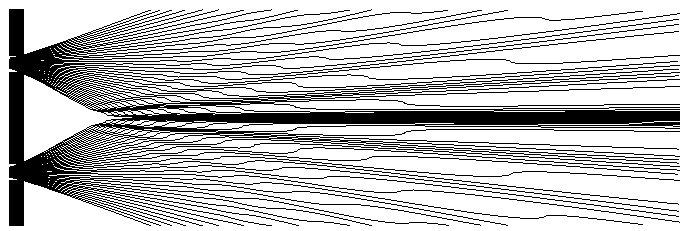
\includegraphics[width=.94\linewidth]{figures/ch08_fig01.pdf}
\caption{二重スリット実験で粒子がたどり得るBohm軌道の一例。Springer Science and Business Mediaのご厚意により、許可を得て\cite{ref480}から転載。}
\end{figure}

Bohm力学では、波動関数は「誘導場」の役割を果たす。すなわち、誘導方程式(8.9)を通じて、波動関数が、粒子が従う速度場を生成する。したがってBohm理論は、Newton力学と同様、軌道に沿う粒子の運動を記述する。しかし、古典力学の力と加速度の法則の代わりに、粒子の運動方程式は今や(8.9)で与えられ、その右辺に入る波動関数$\psi$の変化は、Schrödinger方程式で定まる。

この形式は、二重スリット実験の文脈で明快に示せる\cite{ref037,ref481}。図8.1は、スリットの後方で単一粒子が取り得るBohm軌道の集合を示す。各粒子は、これらの確定した軌道の一つをたどり、したがってスリットの一方を通過する。個々の粒子がどのBohm軌道を取るかは、単にその粒子の初期位置に依存する。したがって、各粒子が、与えられた任意の時刻に同じ波動関数$\psi$で記述されても、粒子は決定論的に異なる確定した軌道をたどる。ゆえにBohm力学は、隠れた変数理論の一例である（2.1.2節参照）。つまり、波動関数$\psi$は系の物理状態の完全な記述ではなく、粒子の常に確定した位置$\boldsymbol q_i(t)$が、隠れた変数の役割を果たす。図8.1を見ると、粒子は明確に非Newton的な経路を取る。粒子軌道は直線ではなく、波動関数$\psi$の振幅が大きい領域に集中する。したがって、スクリーン上で観測される、おなじみの干渉模様の極大と極小を、Bohm軌道の「密度」に直接結びつけることができる。


% 原文 p.356
\hypertarget{srcpage:356}{}\label{srcpage:356}
\subsubsectionlink{基本的実体としての粒子}
Bohm理論は、粒子に基本的な存在論的地位を与えることで批判されてきた。相対論的量子論の根本的な水準で粒子を認めることに反対する、一般的な議論は、しばしばなされている（たとえば\cite{ref482,ref483}参照）\footnote{他方、「量子場のBohm力学」、すなわち量子場の理論をBohm型の枠組みに組み込む理論の提案もある\cite{ref484,ref485}。}。さらに、本節で論じたい点であるが、粒子の現れは連続的なデコヒーレンス過程から導けると論じられ、その結果、粒子に基本的役割を与える必要はないとも主張されている\cite{ref408,ref486,ref487}。中間的尺度や巨視的な系のデコヒーレンスした縮約密度行列が、本質的に常に、位置空間の狭い波束の非真正集団を表すことに基づき、Zeh\cite[190頁]{ref408}は、そのような波束を、個々の「粒子」の位置を表すものとみなせるとする。
\begin{quote}
量子場の測定で観測される粒子的側面（乾板上の点、泡箱中の飛跡、計数器のクリックなど）はすべて、関係する局所的、すなわち部分系の密度行列の、このデコヒーレンスを考慮することによって理解できる。
\end{quote}
もちろん、デコヒーレンスから得られる狭い波束の非真正集団が、個々の粒子の知覚をもたらすと解釈するためには、波束の一つだけが知覚される理由を説明する、追加の解釈の枠組みを与えなければならない。すなわち、デコヒーレンスから生じる非真正集団から個々の項の知覚へ至るためには、何らかの解釈規則を加える必要があり、それゆえ、デコヒーレンスだけで必ずBohmの粒子概念が不要になるわけではない。しかし、基本的実体として粒子を仮定することは不要かもしれないと示唆される。そして、そのような粒子理論を相対論的量子場理論と両立させる困難も考え合わせると、理論の基本的水準に粒子を先験的に仮定するBohmの立場は、重大な挑戦を受けているように見える。

\subsubsectionlink{Bohm軌道とデコヒーレンス}
Bohm力学のよく知られた性質は、その軌道がしばしば著しく非古典的になることである（たとえば\cite{ref037,ref488,ref489}参照）。これは、巨視的水準での準古典的軌道の存在を、Bohm理論がどのように説明できるのかという、重大な問題を生む。


% 原文 p.357
\hypertarget{srcpage:357}{}\label{srcpage:357}
BohmとHiley\cite{ref037}は、巨視的な系による環境粒子ビームの散乱を考えた。この過程はデコヒーレンスを生じさせる\cite{ref007,ref017}。彼らは、この散乱が系の準古典的軌道をもたらすことを示した。またAppleby\cite{ref489}は、孤立系については、Bohm理論は一般に正しい古典極限を与えないことを示した。そこで、環境と、それによるデコヒーレンス効果を含めることが、Bohm力学で準古典的軌道を回復するために役立つかもしれないと提案された\cite{ref486,ref490,ref491,ref492,ref493,ref494}。基本的考えは、デコヒーレンスが作り出す非真正集団における準Newton的な位相空間軌道（たとえば5.2.5節参照）を、Bohm理論の粒子軌道$Q(t)$と結びつけることである。Bacciagaluppi\cite{ref391}が指摘したように、この方法の大きな利点は、同じ方法で量子現象と古典現象の両方を回復できることである。

しかし、Appleby\cite{ref490}の注意深い分析は、デコヒーレンスをもたらす過程が巨視的な系の正しい準古典的Bohm軌道ももたらすのは、ある追加の仮定の下だけであることを示した。Applebyは、初めにエネルギー固有状態に準備された系の、長時間極限の例を述べた。Allori\cite{ref491}、AlloriとZanghì\cite{ref492}、Alloriら\cite{ref493}も、興味深い結果を報告している。これらの著者は、デコヒーレンス効果が、Bohm軌道の古典的性質を保存する役割を果たし得ることを示した。さらに、標準量子力学では、古典性の出現を説明するために狭い波束を維持することが重要であるのに対して、波動関数と配置の両方によるBohm的な系の記述では、高度に非局在化した波動関数から、準古典的振る舞いを導けることを示した。

SanzとBorondo\cite{ref494}は、Bohm力学の枠組みで、デコヒーレンスがある場合の二重スリット実験を調べた。空間的コヒーレンスが完全に失われ、したがって干渉がなくなっても、Bohm理論における粒子の動力学へ影響する非局所的量子相関が残ることを示した。この例は、一般には、デコヒーレンスだけでは、Bohm力学の正しい古典極限を保証するには十分でないことを示している。

\subsectionlink{まとめ}
本章では、各解釈における「確定した量」の、非常に一般的で経験的に適切な定義と説明を実現するため、優先状態の環境誘起超選択が、量子力学の異なる解釈へどのように組み込まれてきたかを示した。
% 原文 p.358
\hypertarget{srcpage:358}{}\label{srcpage:358}
こうして、デコヒーレンスの研究計画は、多くの解釈を長く悩ませてきた悪名高い優先基底問題の解決に、非常に大きな貢献をした。相対状態解釈のような場合には、優先基底の明確な定義がないことが、そのような解釈に対する継続的批判の中心であった。物理的収縮理論やBohm力学のような場合には、優先基底の具体的な形が単に仮定されている。この場合、デコヒーレンスは、仮定される量の特定の選択に、物理的動機を与えることができる。

量子力学の標準解釈の中では、デコヒーレンスは量子測定の結果の問題を解決できないと論じた。私たちには依然として、多数の成分が残される。各成分がよく局在した準古典的なものであるとしても同じである。そして、単一の結果が知覚される理由と仕方を説明するためには、この状況に何かを補うか、あるいは解釈する必要がある。したがって、結果の知覚と一般的な古典性を説明するため、固有値・固有状態リンクを変えたり完全に捨てたり、ユニタリー動力学を修正したりする別の解釈的方法の規則や仮定に、物理的動機を与え、あるいはそれらを反証するために、環境誘起超選択と干渉項の局所的抑制を、大いに利用できることを論じた。

たとえば、その応用のいくつかだけを挙げると、デコヒーレンスは、相対状態解釈における分枝選択の普遍的基準と、観測者の視点から見た分枝間の非干渉についての物理的説明を与えられる。様相解釈では、系へ割り当て得る、経験的に適切な性質の集合を指定するために使える。収縮模型では、自由パラメーター、そしておそらくは縮約機構自体の性質さえも、環境相互作用から導けるかもしれない。Bohm力学で準古典的な粒子軌道を選ぶ助けにもなる。さらに、デコヒーレンスは、異なる解釈の経験的適合性、したがって経験的等価性を保証し得ることが明らかになった。この点から、物理学者Max Tegmarkは、たとえば正統的解釈とEverett解釈の選択が、「純粋に好みの問題となり、おおよそ、数学的言語と人間の言語のどちらを、より根本的だと信じるかに等しくなる」\cite[855頁]{ref495}かもしれないと提案した。

